\documentclass[aspectratio=169,11pt]{beamer}

% ============================================================
% HUST-styled Beamer theme (built from scratch — no official
% HUST .sty/template was available to reuse; colors and the
% dotted decorative pattern are visual approximations of a
% reference HUST deck, not official brand assets. Swap
% \hustred/\hustgold or the logo placeholder below if exact
% brand values become available.)
% ============================================================
\usetheme{default}
\usepackage{fontspec}
\usepackage{tikz}
\usepackage{booktabs}
\usetikzlibrary{calc}

\definecolor{hustred}{HTML}{C8102E}
\definecolor{hustgold}{HTML}{F2A900}
\definecolor{cardgray}{HTML}{F0F0F0}
\definecolor{inkgray}{HTML}{52514E}

\setbeamertemplate{navigation symbols}{}
\setbeamersize{text margin left=0.9cm, text margin right=0.9cm}
\setbeamercolor{background canvas}{bg=white}
\setbeamercolor{normal text}{fg=black}
\setbeamerfont{normal text}{family=\sffamily}
\setbeamercolor{frametitle}{bg=hustred, fg=white}
\setbeamerfont{frametitle}{series=\bfseries, size=\Large}
\setbeamertemplate{itemize items}[circle]
\setbeamercolor{itemize item}{fg=hustred}

% ---- Custom frame title: red bar + page badge + gold rule ----
\setbeamertemplate{frametitle}{%
  \vskip-1pt%
  \makebox[0pt][l]{\hspace*{-0.9cm}%
  
\begin{tikzpicture}[baseline=0pt]
    \useasboundingbox (0,0) rectangle (\paperwidth,1.15cm);
    \fill[hustred] (0,0) rectangle (\paperwidth,1.15cm);
    \node[anchor=west, text=white, font=\bfseries\Large, align=left, text width=\paperwidth-2.6cm] at (0.5cm,0.6cm) {\insertframetitle};
    \node[anchor=east, text=white, font=\normalsize] at ($(\paperwidth,0)+(-0.5cm,0.6cm)$) {\insertframenumber/\inserttotalframenumber};
  \end{tikzpicture}}\par
  \makebox[0pt][l]{\hspace*{-0.9cm}{\color{hustgold}\rule{\paperwidth}{2.2pt}}}\par
  \vskip 0.15cm
}

% ---- Custom footline: text logo lockup + thin rule ----
\setbeamertemplate{footline}{%
  \makebox[0pt][l]{\hspace*{-0.9cm}{\color{hustred!60}\rule{\paperwidth}{0.6pt}}}\par
  \vskip 1pt
  \hspace{0.9cm}%
  \raisebox{0pt}{\tikz\node[fill=hustred, text=white, font=\bfseries\tiny, inner sep=2pt]{H};}%
  \hspace{3pt}{\tiny\color{inkgray} HUST \textbar{} Customer Churn Prediction}%
  \vskip 2pt
}

% ---- Reusable macros: numbered card, stat tile ----
\newcommand{\cardbadge}[1]{\tikz[baseline=-0.65ex]{\node[circle, fill=hustred, text=white, font=\bfseries\small, inner sep=0pt, minimum size=20pt] {#1};}}

\newcommand{\card}[3]{%
  \begin{tikzpicture}
    \node[rounded corners=6pt, fill=cardgray, inner sep=8pt, text width=3.3cm, align=left, anchor=north west] {%
      \cardbadge{#1}\\[6pt]
      {\bfseries\small\color{hustred} #2}\\[3pt]
      {\scriptsize\color{inkgray} #3}%
    };
  \end{tikzpicture}%
}

\newcommand{\stattile}[2]{%
  \begin{tikzpicture}
    \node[rounded corners=6pt, fill=cardgray, inner sep=6pt, minimum width=2.9cm, align=center] {%
      \begin{minipage}{2.5cm}\centering
        {\color{hustred}\bfseries\large #1}\\[0pt]
        {\scriptsize\color{inkgray} #2}
      \end{minipage}%
    };
  \end{tikzpicture}%
}

% ---- Decorative dot spray (TikZ, procedural — no external image) ----
% Must be called *inside* an existing tikzpicture, given a coordinate name,
% e.g. \dotspray{(mycenter)}{hustred} after \coordinate (mycenter) at (...);
\newcommand{\dotspray}[2]{%
  \foreach \r in {0.3,0.7,...,3.3}{
    \foreach \a in {0,20,...,340}{
      \pgfmathsetmacro{\op}{max(0.12,1-\r/3.6)}
      \filldraw[#2, opacity=\op] ($#1+(\a:\r)$) circle (1.3pt);
    }
  }
}

\title{Customer Churn Prediction}
\author{}
\date{}

\begin{document}

% ============================================================
% 1. Title slide
% ============================================================
{
\setbeamertemplate{footline}{}
\begin{frame}[plain]
  \begin{tikzpicture}[remember picture, overlay]
    \coordinate (titledots) at ($(current page.north east)+(-2.6,-2.6)$);
    \dotspray{(titledots)}{hustred}
  \end{tikzpicture}
  \vspace{0.3cm}

  \tikz\node[fill=hustred, text=white, font=\bfseries, inner sep=6pt]{HUST};\\[0.15cm]
  {\scriptsize\color{inkgray} TRƯỜNG ĐẠI HỌC BÁCH KHOA HÀ NỘI\\ HANOI UNIVERSITY OF SCIENCE AND TECHNOLOGY}

  \vspace{0.5cm}
  {\LARGE\bfseries\color{hustred} Customer Churn Prediction}\\[0.3cm]
  {\large\bfseries\color{inkgray} Value-Aware Targeting for Retention Marketing}\\[0.2cm]
  {\normalsize\color{inkgray} RFM features, Logistic Regression, and a business-impact evaluation\\ on the Online Retail II dataset}

  \vspace{0.5cm}
  {\bfseries Group 3 \textbar{} Business Data Analytics -- 10-minute presentation}

  \vspace{0.4cm}
  {\color{hustred!70}\small ONE LOVE. ONE FUTURE}
\end{frame}
}

% ============================================================
% 2. Objective
% ============================================================
\begin{frame}{The Business Problem}
  \begin{columns}[t]
    \column{.33\textwidth}
    \card{1}{Existing customers drive revenue}{Repeat customers already generate most of the revenue -- protecting them matters more than chasing new ones.}
    \column{.33\textwidth}
    \card{2}{Retention is cheaper}{Keeping an at-risk customer costs far less than acquiring a replacement.}
    \column{.33\textwidth}
    \card{3}{Churn = 90 days quiet}{A customer is labeled churned if they make no valid purchase within 90 days of a weekly snapshot.}
  \end{columns}

  \vspace{0.45cm}
  \textbf{Goal:} a weekly churn score per customer -- and a check that acting on it makes business sense.
\end{frame}

% ============================================================
% 3. Insight 1 -- value concentration
% ============================================================
\begin{frame}{Insight 1: Revenue is highly concentrated}
  \begin{columns}[t]
    \column{.5\textwidth}
    \vspace{0.15cm}
    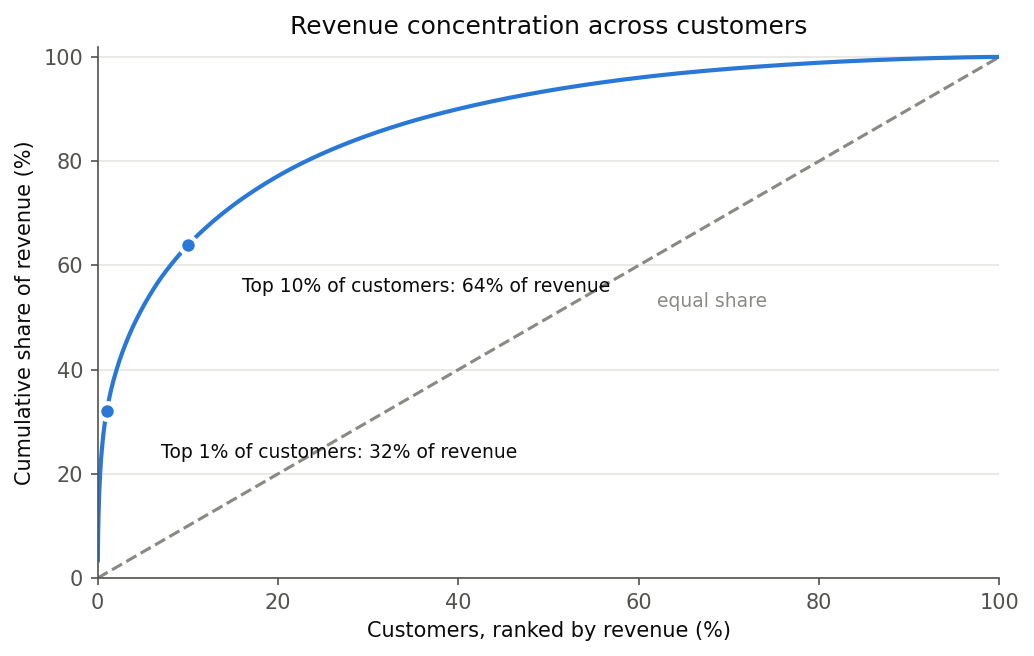
\includegraphics[width=\textwidth]{figures/value_concentration.png}
    \column{.5\textwidth}
    \stattile{32\%}{top 1\% of customers}\\[0.1cm]
    \stattile{52\%}{top 5\% of customers}\\[0.1cm]
    \stattile{64\%}{top 10\% of customers}

    \vspace{0.12cm}
    {\scriptsize\color{inkgray} High-value customers are where retention spend has the most leverage.}
  \end{columns}
\end{frame}

% ============================================================
% 4. Approach (compact)
% ============================================================
\begin{frame}{Our Approach (in brief)}
  \begin{columns}[t]
    \column{.33\textwidth}
    \card{1}{Weekly snapshots}{One row per customer per Monday, only for customers active and not yet lost (recency $\leq$ 136 days).}
    \column{.33\textwidth}
    \card{2}{8 point-in-time features}{RFM, order value, tenure, purchase rhythm and recent activity -- all leakage-safe by construction.}
    \column{.33\textwidth}
    \card{3}{Final model}{Logistic Regression, $C{=}0.01$, trained on every weekly snapshot with per-customer weights -- each choice made on validation.}
  \end{columns}
\end{frame}

% ============================================================
% 5. Results
% ============================================================
\begin{frame}{Model Results}
  \begin{columns}[t]
    \column{.5\textwidth}
    \stattile{0.759}{ROC-AUC (test)}\quad
    \stattile{0.654}{PR-AUC (test)}\\[0.15cm]
    \stattile{1.89}{Lift@10\% (weekly mean)}\quad
    \stattile{0.75}{Precision@10\%}

    \vspace{0.15cm}
    {\scriptsize\color{inkgray} Leads every baseline in all 10 test weeks, with low week-to-week variance.}
    \column{.5\textwidth}
    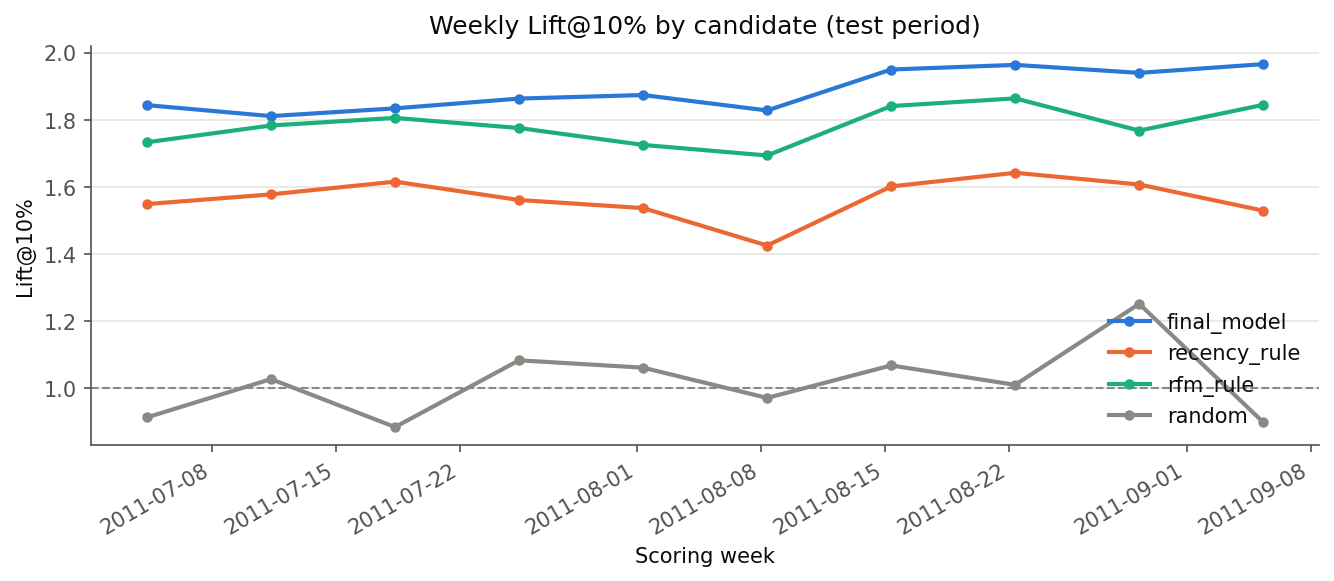
\includegraphics[width=\textwidth]{figures/weekly_lift.png}
  \end{columns}
\end{frame}

% ============================================================
% 6. Insight 2 -- counter-intuitive result
% ============================================================
\begin{frame}{Insight 2: Best Model $\neq$ Most Profitable}
  At the standard 10\% targeting level ($e{=}40\%$, $m{=}35\%$):

  \begin{center}
  \small
  \begin{tabular}{@{}lccc@{}}
    \toprule
    Candidate & Churners caught & Net business impact \\
    \midrule
    \textbf{Churn model} & \textbf{1,831} & \pounds51,506 \\
    RFM rule (hand-built) & 1,732 & \pounds64,616 \\
    Recency rule & 1,521 & \textbf{\pounds70,214} \\
    Random & 986 & \pounds41,626 \\
    \bottomrule
  \end{tabular}
  \end{center}

  \vspace{0.3cm}
  {\color{hustred}\bfseries Counter-intuitive:} the model catches the most churners and wins every predictive metric -- yet ends up the \emph{least} profitable of the three real rules.
\end{frame}

% ============================================================
% 7. Insight 3 -- root cause
% ============================================================
\begin{frame}{Insight 3: Risk $\neq$ Value}
  \begin{columns}[t]
    \column{.55\textwidth}
    Average order value shows only \textbf{weak separation} by churn outcome:
    \begin{center}
    \small
    \begin{tabular}{@{}lcc@{}}
      \toprule
       & Churned & Not churned \\
      \midrule
      Median AOV & \pounds269 & \pounds324 \\
      \bottomrule
    \end{tabular}
    \end{center}
    So ranking purely by churn probability does \emph{not} automatically prioritize high-value customers.
    \column{.45\textwidth}
    The simpler rules (recency, RFM) happen to catch a higher-value subset -- even while catching \emph{fewer} churners overall. This is not a bug: the model optimizes risk, not revenue.
  \end{columns}
\end{frame}

% ============================================================
% 8. Recommendation
% ============================================================
\begin{frame}{Recommendation}
  \begin{columns}[t]
    \column{.5\textwidth}
    \card{1}{Rank by expected value}{Score = P(churn) $\times$ customer value, not churn probability alone -- so targeting optimizes revenue, not just risk.}
    \column{.5\textwidth}
    \card{2}{Pilot with a control group}{This dataset has no past campaign data -- every pound figure shown is a scenario estimate, not an observed outcome.}
  \end{columns}
\end{frame}

% ============================================================
% 9. Summary
% ============================================================
\begin{frame}{Summary: Three Takeaways}
  \begin{enumerate}
    \item Revenue is highly concentrated -- the top 5\% of customers already drive 52\% of it.
    \item The churn model wins on every predictive metric, but \textbf{risk is not value}: at a 10\% target it is less profitable than a simple recency rule.
    \item Recommendation: rank by \textbf{expected value}, not churn probability alone, and validate with a real pilot before scaling.
  \end{enumerate}
\end{frame}

% ============================================================
% 10. Thank you
% ============================================================
{
\setbeamertemplate{footline}{}
\begin{frame}[plain]
  
\begin{tikzpicture}[remember picture, overlay]
    \fill[hustred] (current page.south west) rectangle ($(current page.north west)+(0.38\paperwidth,0)$);
    \coordinate (closedots) at ($(current page.south west)+(0.19\paperwidth,4.2cm)$);
    \begin{scope}
      \clip (current page.south west) rectangle ($(current page.north west)+(0.38\paperwidth,0)$);
      \dotspray{(closedots)}{white}
    \end{scope}
    \node[anchor=south west, xshift=0.4cm, yshift=0.4cm] at (current page.south west) {\tikz\node[fill=white, text=hustred, font=\bfseries, inner sep=6pt]{HUST};};
    \node[anchor=south west, xshift=0.4cm, yshift=0.2cm] at ($(current page.south west)+(0,0.9cm)$) {\scriptsize\color{white} hust.edu.vn \textbar{} fb.com/dhbkhn};
  \end{tikzpicture}
  \begin{tikzpicture}[remember picture, overlay]
    \node[anchor=west, xshift=0.42\paperwidth, yshift=0.3cm] at (current page.west) {%
      \begin{minipage}{0.5\paperwidth}
        {\Huge\bfseries\color{hustred} Thank you!}\\[0.3cm]
        {\Large\color{inkgray} Questions?}
      \end{minipage}%
    };
  \end{tikzpicture}
\end{frame}
}

\end{document}
